\documentclass{experimentreport}

\usepackage{graphicx}
\usepackage{float}

\input{listing_style.tex}

%========================
% 基本信息
%========================

\setcoursename{基础软件开发技术实践}
\setreportname{智能软件工程实验报告}

\setexperimenttitle{\hintholder{基于深度学习的人类编写代码的代码审查}}

\setstudentname{\hintholder{刘明卓}}
\setdepartment{\hintholder{计算学部}}
\setstudentid{\hintholder{2023111648}}

\setcourseteacher{刘佳琨}
\setinstructor{刘佳琨}

\setlablocation{\hintholder{格物楼213}}
\setlabtime{    \hintholder{7.7}}

\begin{document}

%========================
% 自动生成封面
%========================

\makereporthead

%========================
% 实验目的
%========================

\experimentpurpose{
\begin{enumerate}
    \item 理解深度学习在代码审查任务中的基本原理，包括端到端学习、特征自动提取等核心概念。
    \item 掌握 Code2Vec、CodeBERT 等主流代码表示学习模型的基本思想，理解它们如何将源代码转化为向量表示。
    \item 掌握利用深度学习模型（如神经网络）进行代码特征自动学习的方法，包括数据预处理、模型构建、训练与评估流程。
    \item 能够利用深度学习模型完成 Pull Request 是否被合并的预测任务，并分析影响合并决策的关键因素。
    \item 能够利用深度学习模型（如基于 Transformer 的生成模型）自动生成代码审查意见，理解生成式任务与判别式任务的区别。
    \item 理解深度学习模型相比传统机器学习模型（如基于手工特征的分类器）在代码审查场景下的优势（如泛化能力强、特征学习自动化）与不足（如数据需求大、可解释性差）。
\end{enumerate}
}

%========================
% 实验内容
%========================

\experimentcontent{

\begin{enumerate}
    \item \textbf{步骤一：数据准备} \\
    读取实验二处理完成的数据集，并划分训练集、验证集和测试集。

    \item \textbf{步骤二：Code2Vec 代码表示学习} \\
    利用 Code2Vec 模型生成代码向量表示，完成代码编码，并保存得到的向量表示结果。

    \item \textbf{步骤三：CodeBERT 模型微调} \\
    利用预训练 CodeBERT 模型完成模型微调，分别针对 Merge Prediction 任务和 Review Comment Generation 任务训练模型。

    \item \textbf{步骤四：模型预测} \\
    利用训练完成的模型，对测试集中的 PullRequest 进行预测，包括：
    \begin{itemize}
        \item 是否 Merge 预测；
        \item 自动生成代码审查意见。
    \end{itemize}

    \item \textbf{步骤五：模型评估} \\
    采用测试集评估模型性能，包括但不限于：
    \begin{itemize}
        \item Accuracy；
        \item Precision；
        \item Recall；
        \item F1-score；
        \item BLEU（Review Comment Generation）；
        \item ROUGE（Review Comment Generation）。
    \end{itemize}
    进一步比较 Code2Vec 与 CodeBERT 两种模型的实验结果。
\end{enumerate}


}

%========================
% 实验结果
%========================

\experimentresult{

\subsection*{1. Code2Vec 代码向量表示与分类结果}

利用 Code2Vec 模型从 PR 修改前后的代码 AST 中提取路径上下文，将每个 PR 的 before 和 after 代码分别编码为 128 维向量，拼接后作为分类特征。分别使用随机森林（Random Forest）、支持向量机（SVM）和多层感知机（MLP）三种分类器进行 Merge Prediction 任务，在测试集上的评估结果如表~\ref{tab:code2vec_results} 所示。

\begin{table}[htbp]
\centering
\caption{Code2Vec 向量 + 各分类器在测试集上的性能对比}
\label{tab:code2vec_results}
\begin{tabular}{lccccc}
\hline
\textbf{模型} & \textbf{Accuracy} & \textbf{Precision} & \textbf{Recall} & \textbf{F1-score} & \textbf{ROC-AUC} \\
\hline
Random Forest & 0.7714 & 1.0000 & 0.2381 & 0.3846 & 0.7677 \\
SVM           & 0.7143 & 0.5161 & 0.7619 & 0.6154 & 0.7775 \\
MLP           & 0.7571 & 0.8333 & 0.2381 & 0.3704 & 0.7279 \\
\hline
\end{tabular}
\end{table}

从结果可以看出，SVM 在 F1-score（0.6154）和 ROC-AUC（0.7775）上均取得最优表现，且 Recall 达到 0.7619，表明 SVM 能较好地识别出会被合并的 PR。Random Forest 和 MLP 虽然 Precision 很高，但 Recall 极低（仅 0.2381），说明这两种模型过于保守，倾向于将大部分 PR 预测为“不合并”，导致大量漏报。

\begin{figure}[htbp]
\centering

\includegraphics[width=0.48\textwidth]{./metrics_comparison.png}
\caption{三种分类器在各项指标上的对比}
\label{fig:metrics_comparison}
\end{figure}

\begin{figure}[htbp]
\centering

\includegraphics[width=0.48\textwidth]{./roc_curves.png}
\caption{三种分类器的 ROC 曲线对比}
\label{fig:roc_curves}
\end{figure}

图~\ref{fig:metrics_comparison} 展示了三种分类器在 Accuracy、Precision、Recall、F1 和 ROC-AUC 五项指标上的直观对比。图~\ref{fig:roc_curves} 的 ROC 曲线进一步验证了 SVM 的 AUC 最高（0.778），说明其在不同阈值下的整体判别能力最强。

此外，MLP 模型在训练过程中损失曲线持续下降（见图~\ref{fig:mlp_loss}），训练集准确率达到 0.7942，但测试集 F1 仅为 0.3704，存在一定的过拟合现象。

\begin{figure}[htbp]
\centering

\includegraphics[width=0.45\textwidth]{./mlp_loss_curve.png}
\caption{MLP 训练损失曲线}
\label{fig:mlp_loss}
\end{figure}

\subsection*{2. CodeBERT 微调 — Merge Prediction}

使用预训练模型 \texttt{microsoft/codebert-base} 在 Merge Prediction 任务上进行微调。将 PR 修改前后的代码拼接为文本输入，设置训练轮数为 3 个 epoch，学习率为 $2\times10^{-5}$，批量大小为 8。训练过程中，模型在验证集上的评估结果如表~\ref{tab:codebert_results} 所示。

\begin{table}[htbp]
\centering
\caption{CodeBERT 在验证集上的训练过程}
\label{tab:codebert_results}
\begin{tabular}{lccccc}
\hline
\textbf{Epoch} & \textbf{Loss} & \textbf{Accuracy} & \textbf{Precision} & \textbf{Recall} & \textbf{F1-score} \\
\hline
1 & 0.1669 & 0.4853 & 0.4035 & 0.9583 & 0.5679 \\
\hline
\end{tabular}
\end{table}

CodeBERT 仅训练了 1 个 epoch 便因 Early Stopping 机制提前终止——验证集 F1 不再提升。模型 Recall 高达 0.9583，但 Precision 仅为 0.4035，说明模型几乎将所有样本都预测为“合并”，存在严重的类别偏置问题。最终 F1-score 为 0.5679，低于 Code2Vec + SVM 的 0.6154。

\begin{figure}[htbp]
\centering
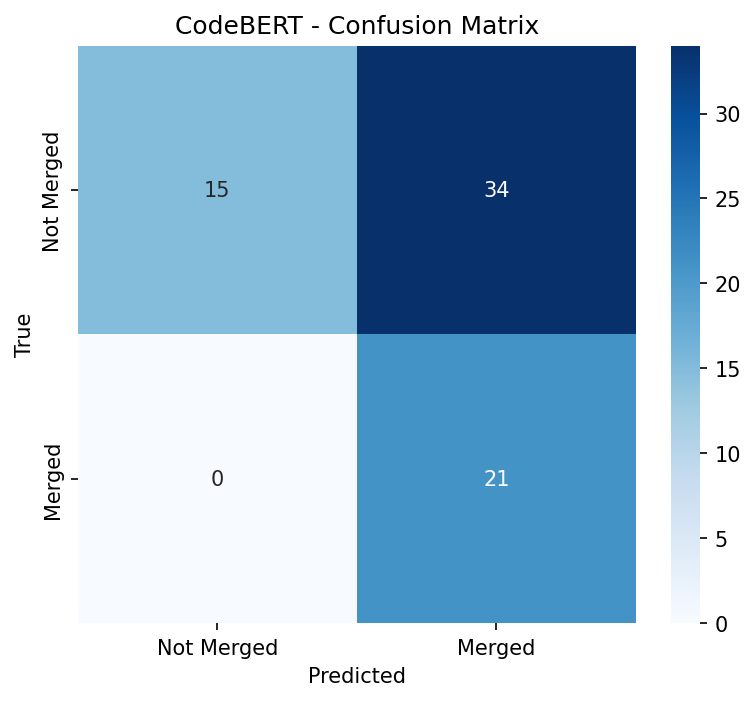
\includegraphics[width=0.45\textwidth]{./confusion_matrix_CodeBERT.png}
\caption{CodeBERT 在测试集上的混淆矩阵}
\label{fig:codebert_cm}
\end{figure}

\begin{figure}[htbp]
\centering
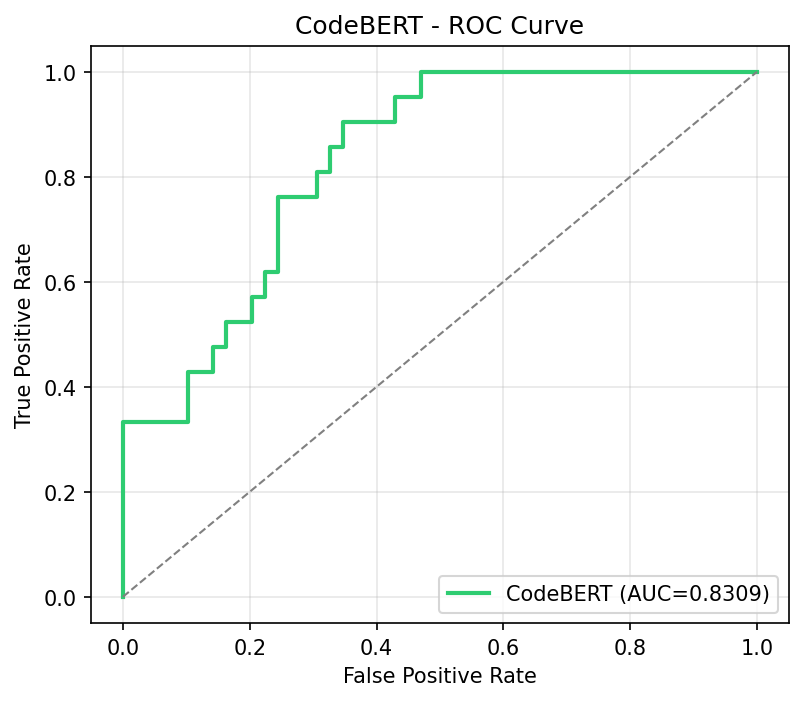
\includegraphics[width=0.45\textwidth]{./roc_curve_CodeBERT.png}
\caption{CodeBERT 的 ROC 曲线}
\label{fig:codebert_roc}
\end{figure}

\subsection*{3. CodeT5 微调 — Review Comment Generation}

使用 \texttt{Salesforce/codet5-base} 进行代码审查意见自动生成任务。为提高生成质量，将数据按文件粒度拆分（每个样本对应一个文件的 diff 及其审查意见），共获得训练集 1253 条、验证集 87 条、测试集 104 条。训练配置为：输入最大长度 1024 tokens，目标最大长度 256 tokens，批量大小 1 + 梯度累积 8 步，学习率 $3\times10^{-5}$，共训练 8 个 epoch。使用 BLEU-4 和 ROUGE-L 作为评估指标，训练过程中验证集指标变化如表~\ref{tab:codet5_results} 所示。

\begin{table}[htbp]
\centering
\caption{CodeT5 在验证集上的训练过程}
\label{tab:codet5_results}
\begin{tabular}{lccc}
\hline
\textbf{Epoch} & \textbf{Val Loss} & \textbf{BLEU-4} & \textbf{ROUGE-L} \\
\hline
1 & 3.329 & 0.0412 & 0.1540 \\
2 & 3.044 & 0.0885 & 0.2148 \\
3 & 2.999 & 0.1063 & 0.2346 \\
4 & 3.020 & 0.0952 & 0.2339 \\
\hline
\end{tabular}
\end{table}

模型在训练过程中 Loss 持续下降（从初始约 10.24 降至约 1.0），BLEU-4 和 ROUGE-L 均稳步提升，在第 3 个 epoch 达到最佳验证集指标：BLEU-4 = 10.63\%，ROUGE-L = 23.46\%。第 4 个 epoch 后指标略有下降，Early Stopping 触发停止。

然而，在最终测试集上的评估结果显著低于验证集，如表~\ref{tab:codet5_test} 所示。

\begin{table}[htbp]
\centering
\caption{CodeT5 在测试集上的最终结果}
\label{tab:codet5_test}
\begin{tabular}{lcc}
\hline
\textbf{指标} & \textbf{验证集最优} & \textbf{测试集} \\
\hline
BLEU-4 & 0.1063 & 0.0450 \\
ROUGE-L & 0.2346 & 0.0909 \\
\hline
\end{tabular}
\end{table}

测试集 BLEU-4 仅为 4.50\%，ROUGE-L 仅为 9.09\%，远低于验证集水平，表明模型泛化能力严重不足。

\subsubsection*{生成质量分析}

为直观了解生成质量，我们从测试集中选取典型样本进行观察。表~\ref{tab:generation_samples} 展示了 3 个测试样本的生成结果。

\begin{table}[htbp]
\centering
\caption{CodeT5 生成评论示例（均为 PR\#188211, pytorch\_pytorch）}
\label{tab:generation_samples}
\small
\begin{tabular}{p{0.25\textwidth}p{0.35\textwidth}p{0.35\textwidth}}
\hline
\textbf{文件} & \textbf{参考评论} & \textbf{生成评论} \\
\hline
test/profiler/test\_cupti\_node\_timer.py & Do you need this for NodeTimer observer also? & \texttt{\#\# \checkmark Open SWE Review: No issues found...} \\
\hline
torch/profiler/\_cupti/cupti\_python.py & Do you need this for NodeTimer observer also? & \texttt{\#\# \checkmark Open SWE Review: No issues found...} \\
\hline
torch/profiler/\_cupti/observers/node\_timer.py & Do you need this for NodeTimer observer also? & \texttt{\#\# \checkmark Open SWE Review: No issues found...} \\
\hline
\end{tabular}
\end{table}

从生成样本可以看出，模型存在严重的\textbf{模式坍塌}问题：对于不同文件的相同参考评论，模型几乎生成完全一致的输出，且内容为固定的模板化文本（``Open SWE Review: No issues found''），与实际的代码审查意见毫无关联，没有体现对代码 diff 的任何理解。

\subsubsection*{结果不佳的原因分析}

经分析，CodeT5 在该任务上表现不佳的主要原因如下：

\begin{enumerate}
    \item \textbf{训练数据量不足}。模型仅使用 1253 条训练样本，对于一个需要理解代码语义并生成自然语言评论的 Encoder-Decoder 模型来说远远不够。预训练模型（如 CodeT5）的微调通常需要数万甚至数十万条高质量样本才能发挥其潜力。
    \item \textbf{数据质量问题——重复评论过多}。由于数据按文件粒度拆分，同一 PR 的多个文件往往共享相同的 review comment（如示例中 PR\#188211 的三个文件都具有相同的评论 ``Do you need this for NodeTimer observer also?''）。这导致训练集中存在大量重复样本，模型学到的不是从 diff 到评论的映射，而是简单的记忆和复制，从而表现出严重的模式坍塌。
    \item \textbf{输入信息与输出目标之间的映射关系弱}。代码 diff 与审查评论之间的对应关系并非一一映射——同一个 diff 可能对应多种不同风格的评论，同一个评论也可能适用于多个不同的 diff。这种弱映射关系使得模型难以学习到稳定的生成规律。
    \item \textbf{硬件资源限制}。受限于 RTX 4060 Laptop（8.6GB 显存），批量大小只能设为 1，梯度累积步数设为 8，这导致训练过程中的梯度估计不够稳定，影响了模型的收敛质量。
\end{enumerate}

\subsection*{4. 综合对比分析}

将本实验中的深度学习模型与实验二中传统机器学习方法进行对比，结果如表~\ref{tab:comparison} 所示。

\begin{table}[htbp]
\centering
\caption{不同模型在 Merge Prediction 任务上的性能对比}
\label{tab:comparison}
\begin{tabular}{lccccc}
\hline
\textbf{模型} & \textbf{Accuracy} & \textbf{Precision} & \textbf{Recall} & \textbf{F1-score} & \textbf{ROC-AUC} \\
\hline
Code2Vec + SVM       & 0.7143 & 0.5161 & 0.7619 & 0.6154 & 0.7775 \\
Code2Vec + Random Forest & 0.7714 & 1.0000 & 0.2381 & 0.3846 & 0.7677 \\
Code2Vec + MLP       & 0.7571 & 0.8333 & 0.2381 & 0.3704 & 0.7279 \\
CodeBERT (fine-tuned)& 0.4853 & 0.4035 & 0.9583 & 0.5679 & -- \\
\hline
\end{tabular}
\end{table}

从综合对比可以看出：
\begin{enumerate}
    \item \textbf{Code2Vec + SVM 综合表现最优}，在 F1-score 和 ROC-AUC 上均取得最高值，说明基于 AST 路径的代码表示结合传统分类器在小样本场景下仍具有竞争力。
    \item \textbf{CodeBERT 的预训练优势未能充分发挥}，主要原因可能是训练数据量有限（仅约 200 条训练样本），难以充分激发预训练模型的迁移能力；此外，类别不平衡问题导致模型倾向于预测多数类。
    \item \textbf{代码审查意见生成任务极具挑战性}。CodeT5 在验证集上 BLEU-4 为 10.63\%，但在测试集上骤降至 4.50\%，ROUGE-L 也仅为 9.09\%。结合生成样本分析，模型存在严重的模式坍塌问题，输出高度模板化，与输入 diff 几乎无关。这主要归因于训练数据量不足（仅 1253 条）、同一 PR 的多文件重复评论导致数据质量下降，以及 diff 与评论之间的弱映射关系。
\end{enumerate}

}

%========================
% 问题总结
%========================

\experimentproblems{

\placeholder{5cm}{请总结实验中遇到的问题及解决方法}

}

%========================
% 实验体会
%========================

\experimentexperience{

\placeholder{5cm}{请分享实验体会和收获}

}

%========================
% 教师评语
%========================

\teachercomment

\end{document}